\documentclass[../main.tex]{subfiles}
\begin{document}

Procediamo a fare un'introduzione ai dataset storici che hanno contribuito alla ricerca in campo VQA prima di presentare e analizzare il KvasirVQA.

\section{Dataset storici}

\subsection{VQA v1}

Il dataset \textit{VQA v1} viene proposto contestualmente al primo paper di ricerca sull'argomento \cite{DBLP:journals/corr/AntolALMBZP15}, combinando immagini sia astratte, ovvero raffiguranti paesaggi artificiali e stilizzati, sia reali e provenienti dal dataset \textit{Microsoft Common Objects in Context} (MSCOCO) \cite{lin2015microsoftcococommonobjects} con domande e risposte generate da annotatori umani per la sua componente testuale, proponendo una vasta gamma di domande, dalle risposte binarie (Sì/No) a quesiti aperti e numerici.
Parallelamente viene proposta una prima metrica per la valutazione di modelli specializzati in questo task che definisce l'\textit{accuracy} del modello con la seguente formula:

\begin{equation}
    \text{accuracy} = \min\left(\frac{\text{\#humans that provided that answer}}{3}, 1\right)
    \label{eq:accuracy}
\end{equation}

Basando la valutazione del modello in base alla percentuale di annotatori che hanno risposto allo stesso modo alla domanda.

Nonostante la sua importanza, il dataset \textit{VQA v1} presentava alcune limitazioni significative, come una distribuzione non bilanciata delle domande, permettendo ai modelli di ottenere buoni risultati sfruttando bias nei dati, senza una reale comprensione visiva.

Il \textit{VQA v1} ha gettato le basi per lo sviluppo di dataset più avanzati, come il \textit{VQA v2}, che ha affrontato molte delle sue criticità per fornire una valutazione più rigorosa delle capacità dei modelli.

\subsection{Dataset VQA v2}

Il dataset \textit{VQA v2} \cite{DBLP:journals/corr/GoyalKSBP16} è stato rilasciato come evoluzione della versione originale \textit{VQA v1}, ed è stato progettato per andare incontro ad alcune delle limitazioni emerse dalla prima versione.

Il dataset \textit{VQA v2} contiene circa 265.000 immagini provenienti da \textit{MSCOCO}, ognuna associata a domande e risposte multiple. Ogni domanda è bilanciata da coppie di immagini che condividono la stessa domanda ma hanno risposte diverse, al fine di ridurre il bias nei dati. Ad esempio, una domanda sulla quantità di animali presente nell'immagine può avere risposte diverse a seconda della scena mostrata.

Il dataset include oltre 1,1 milioni di domande e circa 11 milioni di risposte raccolte tramite annotazioni umane. Le domande spaziano tra diverse tipologie, come:
\begin{itemize}
    \item \textbf{Domande binarie}: Richiedono una risposta \textit{Sì} o \textit{No}.
    \item \textbf{Domande numeriche}: Prevedono risposte sotto forma di conteggio.
    \item \textbf{Domande aperte}: Richiedono risposte descrittive, come nomi di oggetti o azioni.
\end{itemize}

Il bilanciamento introdotto in \textit{VQA v2} ha migliorato significativamente la qualità delle valutazioni dei modelli, riducendo la possibilità di ottenere alte performance sfruttando semplici bias nei dati. 
Questo rende il dataset particolarmente adatto per testare modelli di VQA che si basano su una comprensione reale delle relazioni tra testo e immagine.

\subsection{Visual Genome}

Il dataset \textit{Visual Genome} \cite{DBLP:journals/corr/KrishnaZGJHKCKL16} contiene circa 108.000 immagini annotate con una vasta gamma di informazioni, incluse relazioni tra oggetti, attributi e domande con risposte generate da annotatori umani.

Oltre alle domande e risposte, Visual Genome offre annotazioni dettagliate a livello di oggetto e di scena, includendo descrizioni, relazioni semantiche e attributi, fornendo un contesto più ricco rispetto a dataset come \textit{VQA v2}. Questa granularità lo rende particolarmente utile per addestrare modelli in grado di catturare relazioni complesse tra gli elementi visivi.

Grazie alla combinazione di annotazioni visive e testuali, Visual Genome è stato ampiamente utilizzato per migliorare le capacità di ragionamento visivo nei modelli di VQA, soprattutto per il loro addestramento su domande che richiedono una comprensione contestuale delle immagini.

\subsection{Graph-based Question Answering (GQA)}

Il dataset \textit{(GQA)} \cite{liang2021graghvqalanguageguidedgraphneural} è progettato per domande strutturate logicamente, basandosi su rappresentazioni grafiche delle scene visive. Contiene oltre 1,7 milioni di domande generate automaticamente, derivanti da 113.000 immagini annotate.

Ogni immagine è rappresentata da un grafo di scene che include oggetti, attributi e relazioni spaziali. Le domande sono costruite per riflettere percorsi logici che attraversano i nodi del grafo, rendendo il task particolarmente complesso.

GQA è stato progettato per migliorare le capacità di ragionamento strutturato dei modelli, rendendolo un riferimento importante per valutare come il ragionamento basato su strutture come i grafi si posizioni a livello di performance rispetto ad altre tecniche.

\subsection{PathVQA}

Il dataset \textit{PathVQA} \cite{he2020pathvqa30000questionsmedical} è uno dei pochi dataset specificamente progettati per il VQA in ambito medico. È composto da circa 32.800 immagini patologiche accompagnate da domande che richiedono competenze diagnostiche specialistiche.

Le domande riguardano anomalie, caratteristiche visive e dettagli clinici presenti nelle immagini. La struttura del dataset è pensata per valutare la capacità dei modelli di rispondere correttamente a domande basate su conoscenze mediche.

Volendo fare un confronto critico, PathVQA rappresenta un riferimento diretto per il KvasirVQA, condividendo un focus simile sul contesto medico. Tuttavia, KvasirVQA si distingue per il suo focus sull'endoscopia gastrointestinale.

\subsection{ScienceQA}

Nel contesto del VQA nel dominio scientifico, è sicuramente utile menzionare il dataset \textit{ScienceQA} \cite{lu2022learnexplainmultimodalreasoning}, sviluppato per affrontare il problema del ragionamento multimodale combinando informazioni provenienti da testo, immagini e conoscenze strutturate per rispondere a domande educative. 

ScienceQA contiene oltre 21.000 domande tratte da materiali educativi di scienze, organizzate in 26 categorie (biologia, chimica, fisica, ecc.) e distribuite su tre livelli educativi (elementare, medio, avanzato). Ogni domanda è accompagnata da:
\begin{itemize}
    \item Un'immagine correlata che arricchisce il contesto visivo.
    \item Risposte multiple.
    \item Spiegazioni dettagliate che delineano il ragionamento necessario per raggiungere la risposta corretta.
\end{itemize}

Il lavoro presentato si concentra sull'integrazione di fonti multimodali per rispondere alle domande. In particolare, il modello proposto utilizza tecniche avanzate come il \textbf{Multimodal Chain-of-Thought Reasoning}, che simula il processo di ragionamento umano combinando contenuti testuali e visivi con conoscenze esterne, tecnica che verrà approfondita nel prossimo capitolo e che sarà impiegata per lo studio delle prestazioni di alcuni modelli generativi sul KvasirVQA.

Ad esempio, il modello potrebbe integrare informazioni testuali e visive per rispondere a domande relative alla funzione di un organo evidenziato in un'immagine, fornendo risposte basate su conoscenze scientifiche consolidate.

ScienceQA offre un banco di prova per testare la capacità dei modelli di risolvere problemi complessi che richiedono non solo la comprensione visiva, ma anche il ragionamento e la conoscenza scientifica. Questo lo distingue da dataset generici di VQA, focalizzandosi su domande che richiedono una fusione profonda delle modalità e un metodo di approccio al problema sicuramente più simile a quello umano.

Il concetto di \textbf{Multimodal Chain-of-Thought Reasoning} esplorato in ScienceQA rappresenta una direzione promettente per l'applicazione al dominio medico. In particolare, le tecniche utilizzate per guidare il ragionamento attraverso spiegazioni strutturate possono ispirare nuove strategie per migliorare le performance su dataset che sfruttano tecniche simili.

\section{KvasirVQA}

Passiamo adesso ad un'introduzione del KvasirVQA con a seguire un'analisi approfondita per la contestualizzazione.

\subsection{Introduzione a KvasirVQA}

Il dataset KvasirVQA è stato creato per affrontare una lacuna significativa nella ricerca sul VQA medico, offrendo dati specifici per immagini diagnostiche. 
Derivato dai dataset HyperKvasir \cite{borgli2020hyperkvasir} e Kvasir-Instrument \cite{borgli2020hyperkvasir}, il KvasirVQA \cite{gautam2024kvasirvqa} si distingue per l'integrazione di immagini mediche e quesiti strutturati, concepiti per supportare la diagnosi e il rilevamento di anomalie in un contesto clinico altamente specializzato.
Il KvasirVQA è stato utilizzato in questa tesi come punto di partenza per lo studio sperimentale, senza interventi diretti nella sua raccolta o annotazione, per indagare gli effetti delle variazioni sui modelli affermati nel campo del VQA.

Nel presente capitolo verranno analizzate in dettaglio le caratteristiche principali del dataset, la sua rilevanza per il task e il suo ruolo specifico nello studio sperimentale condotto.

\subsection{Origine}

Rilasciato a settembre 2024, il dataset KvasirVQA combina immagini provenienti dai dataset HyperKvasir e Kvasir-Instrument, integrando le caratteristiche di entrambi per fornire un insieme completo e diversificato di dati visivi.

HyperKvasir comprende immagini e video di ispezioni del tratto gastrointestinale corredati da annotazioni relative sia a ritrovamenti anomali che a landmark anatomici, utili per la localizzazione durante le procedure endoscopiche. 
Tuttavia, presenta alcune limitazioni, tra cui uno sbilanciamento nella distribuzione delle classi e la mancanza di annotazioni dettagliate per molte categorie. 
Un'analisi preliminare ha rivelato che la maggior parte delle immagini annotate appartiene alla classe "Polipo", riflettendo la maggiore frequenza di questi ritrovamenti rispetto ad altre anomalie. 
Inoltre, le annotazioni relative alla posizione degli oggetti (ad esempio, bounding-box) sono disponibili solo per i polipi, a causa delle difficoltà nell'isolare altre tipologie di anomalie e della presenza di etichette che descrivono l'immagine nel suo complesso, come l'indice Boston Bowel Preparation Scale (BBPS).

Kvasir-Instrument, invece, si concentra su immagini contenenti strumenti medici come pinze da biopsia e sonde, fornendo annotazioni precise tramite bounding-box per localizzare questi strumenti. Questa caratteristica arricchisce il dataset KvasirVQA con informazioni visive fondamentali per applicazioni diagnostiche e interventistiche.

La combinazione di queste risorse rende il dataset KvasirVQA particolarmente adatto a task multimodali come il Visual Question Answering, grazie alla varietà e complessità delle immagini e delle annotazioni fornite. 
Tuttavia, alcune limitazioni ereditarie, come lo sbilanciamento tra le classi e la disponibilità limitata di bounding-box per determinate categorie, hanno influenzato la configurazione degli esperimenti descritti in questa tesi. 
In particolare, alcuni degli approcci adottati si basano sull'uso di features globali, evitando l'introduzione di meccanismi di attenzione complessi.

\subsection{Statistiche e Caratteristiche}

La componente testuale, composta da domande e risposte, è stata sviluppata con il contributo di esperti nel campo della gastroenterologia, includendo una varietà di formati, come domande a risposta multipla, binaria (Sì/No) e altre tipologie.

La distribuzione delle immagini divisa per origine è la seguente:

\begin{table}[H]
    \centering
    \begin{tabular}{|l|c|l|}
    \hline
    \textbf{Categoria} &
    \textbf{N} &
    \textbf{Sorgente} \\ \hline
    Normal             & 2500            & HyperKvasir                   \\ \hline
    Polyps             & 1000            & HyperKvasir                   \\ \hline
    Esophagitis        & 1000             & HyperKvasir                   \\ \hline
    Ulcerative Colitis          & 1000             & HyperKvasir             \\ \hline
    Instrument   &   1000    &   Kvasir-Instrument \\ \hline
    Totale      &       6500        & \\ \hline
    \end{tabular}
    \caption{Distribuzione immagini ricavata da \cite{gautam2024kvasirvqa} con relativo dataset di origine e cardinalità}
    \label{tab:my_label}
\end{table}

La \textit{label} "Normal", in particolare, fa riferimento a delle immagini in cui non sono presenti anormalità o segni distintivi di alcune patologie, ma che semplicemente danno delle informazioni sulla posizione specifica in cui ci si trova all'interno del tratto GI. Tra queste, troviamo ad esempio \textit{cecum} e \textit{ileum}, ovvero l'intestino cieco e ileo. 
La presenza di immagini etichettate come "Normal" consente di addestrare i modelli a distinguere scenari diagnostici complessi da quelli standard, migliorando la loro capacità di generalizzazione e identificazione di patologie.

Per ciascuna delle 6500 immagini presenti, sono state generate sei coppie di domande e risposte, distribuite tra le principali macro-categorie considerate. 
A seguire è riportata una tabella riassuntiva, tratta da \cite{gautam2024kvasirvqa}, che offre una panoramica generale sulla componente testuale del dataset.

\begin{table}[H]
\centering
\begin{tabular}{|>{\centering\arraybackslash}p{3cm}|>{\centering\arraybackslash}p{6cm}|>{\centering\arraybackslash}p{5cm}|}
\hline
\textbf{Type} & \textbf{Question} & \textbf{Answer Options} \\ \hline
Yes/No & Have all polyps been removed? / Is this finding easy to detect? / Is there text? / Is there a green/black box artefact? / Does this image contain any finding? / What type of polyp is present? & No / Yes / Not relevant \\ \hline
Choice (Single)  & What type of procedure is the image taken from? & Paris Ip / Paris IIa / Paris Is / Capsule Endoscopy / Colonoscopy / Gastroscopy \\ \hline 
Choice (Single)  & What is the size of the polyp? & $<$5mm / 5-10mm / 11-20mm / $>$20mm \\ \hline 
Choice (Multiple) & Are there any abnormalities in the image? & Oesophagitis, Ulcerative Colitis, Short-Segment Barretts, Barretts, Polyp, Hemorrhoids \\ \hline
Choice (Multiple) & Are there any anatomical landmarks in the image? & Ileum, Z-Line, Cecum, Pylorus \\  \hline
Choice (Multiple) & Are there any instruments in the image? & Tube, Metal Clip, Polyp Snare, Injection Needle, Biopsy Forceps \\ \hline
Choice (Color) & What color is the abnormality? & landmark: grey, flesh, pink, black, orange, etc. \\ \hline
Choice (Color) & What color is the anatomical landmark? & pink, red, etc. \\ \hline
Location & Where in the image is the abnormality? / Where in the image is the instrument? / Where in the image is the anatomical landmark? & Upper-Left / Upper-Center / Upper-Right / Center-Left / Center / Center-Right / Lower-Left / Lower-Center / Lower-Right \\ \hline
Numerical Count & How many findings are present? / How many polyps are in the image? / How many instruments are in the image? & [0-inf] \\ \hline
\end{tabular}
\caption{Domande, categorizzate per tipologia, e relative risposte dal KvasirVQA\cite{gautam2024kvasirvqa}}
\label{tab:question_types}
\end{table}

Le domande presenti nel dataset sono diversificate e comprendono formati che spaziano da risposte binarie al conteggio delle anomalie visibili nell'immagine, fino al rilevamento di artefatti specifici, come scritte o riquadri generati dal software utilizzato durante le ispezioni del tratto gastrointestinale. Questa varietà di domande riveste un ruolo cruciale, poiché consente di valutare la capacità dei modelli di comprendere il contenuto visivo, identificare gli elementi di interesse e analizzare il processo attraverso cui il modello osserva e interpreta le immagini.

\subsection{Analisi, limiti e trattamento dei dati}

L'analisi approfondita del dataset KvasirVQA ha messo in evidenza alcune criticità rilevanti. Tra queste, è emersa per esempio la presenza di dati nulli all'interno dei metadati, che aggregano domande e risposte associate a ciascuna immagine, e una distribuzione sbilanciata delle risposte uniche, con alcune categorie sovrarappresentate rispetto ad altre. 
Questi aspetti, pur rappresentando delle limitazioni, offrono spunti di riflessione sulle peculiarità del dataset, che saranno approfonditi nelle sezioni successive.

\subsubsection{Imprecisioni testuali}

Sono emerse delle incongruenze riguardanti le annotazioni di alcune domande o risposte, probabilmente dovute a errori di battitura o sviste, per esempio:

\begin{itemize}
    \item Alcune righe riportano la dicitura "instrumnets" piuttosto che "instruments;
    \item Alcune righe riportano la dicitura "$>$20" piuttosto che "$>$20mm";
    \item Alcune righe riportano la dicitura "rigth" piuttosto che "right".
\end{itemize}

Si suppone che queste impurità verranno corrette con dei rilasci futuri di versioni più ricche e rifinite del dataset. 
Per l'attività di ricerca della tesi, queste righe sono state pulite e una copia del file in formato CSV bonificato verrà mantenuta ed utilizzata per addestramenti e test.

\subsubsection{Presenza di dati nulli}

All'interno del file contenente i metadati sono state ritrovate cinquantuno righe con dati nulli, che reputiamo un refuso del dataset e sono state eliminate prima di ulteriori elaborazioni, modifiche o considerazioni sul dataset. 

La rimozione ha portato il numero effettivo di righe del dataset a 58.798, permettendoci di proseguire nella nostra ricerca.

\subsubsection{Domande}

Come possiamo vedere dalla tabella presentata precedentemente, sono presenti in totale diciannove domande distinte all'interno del dataset e con riferimenti ai tre principali punti di interesse che possiamo ritrovare nelle foto, ovvero anomalie, strumenti e \textit{landmark} anatomici.
Nel KvasirVQA possiamo trovare dunque domande riguardo:

\begin{itemize}
    \item Domande relative al posizionamento;
    \item Presenza nell'immagine;
    \item Conteggio degli oggetti d'interesse;
    \item Presenza artefatti software;
    \item Domande relative a caratteristiche dei ritrovamenti.
\end{itemize}

È stata inoltre verificata una lunghezza massima in parole di tredici per le domande, dato utile per stabilire eventuali parametri per la tokenizzazione della componente testuale.

\subsubsection{Risposte e Data Augmentation}

Prima della bonifica testuale, sono state rilevate all'interno del dataset 501 risposte distinte alle domande presenti, diventate 469 dopo la correzione delle imprecisioni che sono state notate durante lo studio del KvasirVQA. 
Parallelamente all'osservazione sulle 469 risposte uniche, è stato rilevato quello che possiamo considerare un vocabolario di, in totale, 58 opzioni uniche combinabili ad esempio nelle risposte a domanda multipla. 
Dato l'alto numero di risposte diverse, è stata ipotizzata una distribuzione sbilanciata di queste all'interno dei dati. 
Nonostante non sia totalmente rappresentativo della distribuzione delle risposte uniche, possiamo comprendere meglio lo sbilanciamento con il seguente grafico delle frequenze dei singoli vocaboli nelle risposte:

\begin{figure}[H]
    \centering
    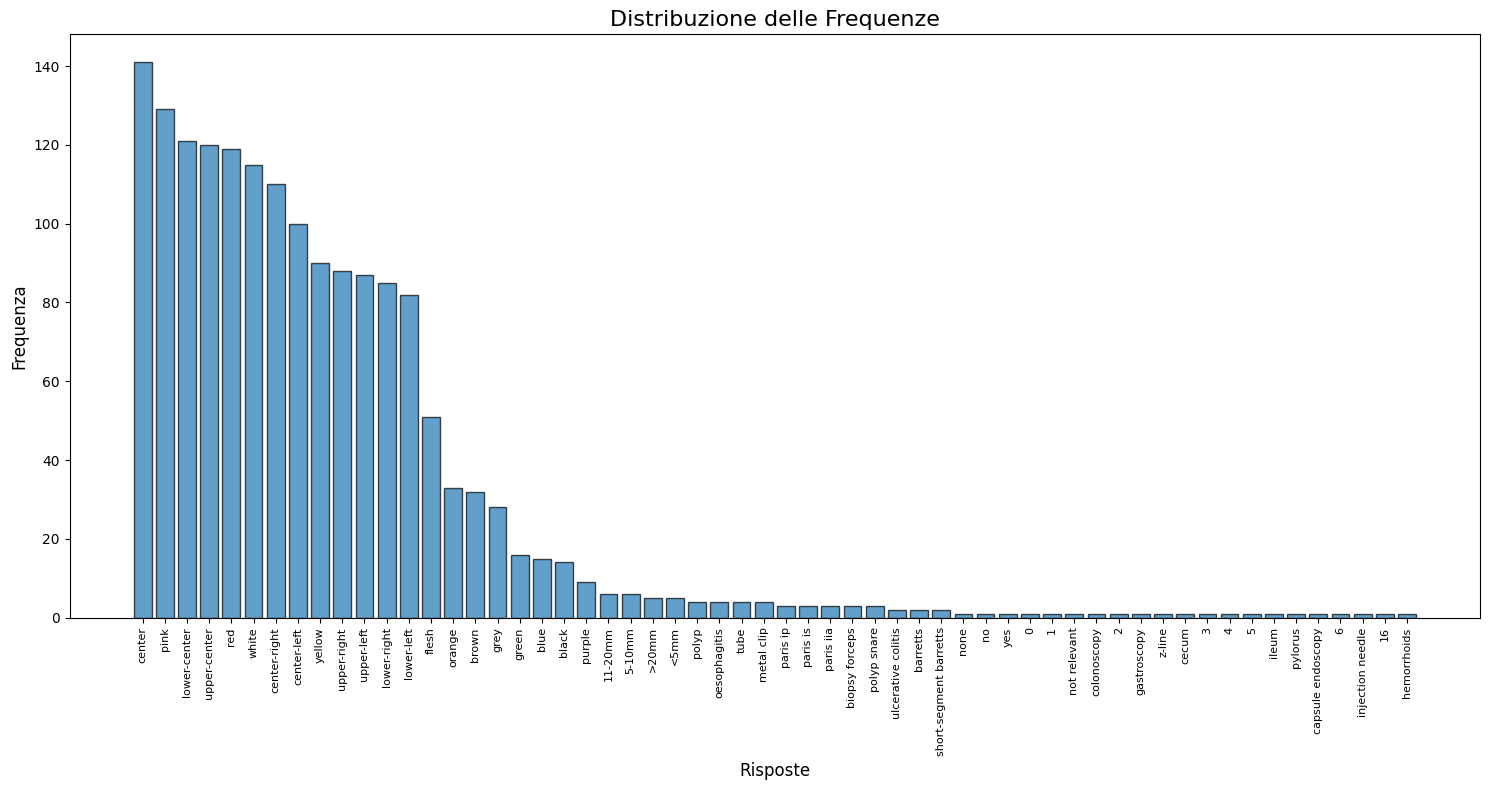
\includegraphics[width=1\linewidth]{static/grafico_frequenze.png}
    \label{fig:enter-label}
\end{figure}

Questo dato è stato di particolare rilevanza nel trattamento del problema in forma chiusa, dal momento che è stato necessario generare sinteticamente nuovi dati a partire da quelli già presenti, distinguendo però l'operazione in due sotto-operazioni distinte, ovvero: \textit{data augmentation} per righe con domande relative alla posizione, e \textit{data augmentation} per tutti gli altri tipi di domanda.
Comunemente a entrambe le procedure è stato fatto in modo che ogni risposta comparisse comunque in almeno otto righe del dataset, così da fornire un minimo esempio, seppur esiguo, al modello, da cui imparare per una corretta classificazione riguardo le coppie di domande e risposte meno frequenti.
Considerando una già menzionata soglia minima di otto righe come frequenza per ogni risposta, sono state generate in totale 2096 nuove righe.
Sebbene la soglia sia esigua, per limitazioni computazionali non è stato possibile fornire una significativa rappresentazione a ognuna delle 496 risposte singole. 
Tuttavia, ipotizziamo che l'augmentation delle righe contenenti le risposte combinate possa essere una base solida.
Le osservazioni sulla distribuzione dei dati e sulle frequenze sono state fondamentali, dal momento che da queste è scaturita la proposta sperimentale di porre il problema nella forma di un task di classificazione multilabel, approccio che verrà approfondito nel capitolo successivo.

\subsubsection{Domande posizionali}

Per quanto riguarda le domande posizionali, sono state applicate due trasformazioni distinte dal \textit{framework PyTorch}:

\begin{itemize}
    \item \textit{ColorJitter}, modificando i parametri dell'immagine come luminosità, contrasto e saturazione con una variazione massima del dieci per cento, e la gradazione (\textit{hue}) del cinque per cento;
    \item \textit{GaussianBlur} per introdurre rumore all'interno delle immagini.
\end{itemize}

\subsubsection{Altre domande}

Per il resto delle domande, sono state applicate le seguenti trasformazioni:

\begin{itemize}
    \item \textit{RandomHorizontalFlip}, ovvero un ribaltamento orizzontale dell'immagine con probabilità che può avvenire con una probabilità p=0.5;
    \item \textit{RandomRotation}, con una rotazione minima tra 0\degree e 270\degree.
\end{itemize}

\section{Conclusioni}

Il KvasirVQA è un passo in avanti importante in ambito medico grazie al suo contributo nel dominio dei dati relativi al tratto gastrointestinale, sia per quanto riguarda il solo task del VQA, che è stato il focus della tesi, sia per altri task come l'\textit{Image Captioning} e la generazione di immagini sintetiche. 
Non escludiamo che possa avere una rilevanza anche maggiore in futuro, con il rilascio di versioni ulteriormente arricchite e maggiormente bilanciate, con un supporto maggiore da parte di esperti gastroenterologi e con l'applicazione da parte di modelli che utilizzino architetture e tecnologie innovative e più evolute rispetto a quelle attualmente esistenti.
Il dataset KvasirVQA rappresenta un passo avanti rispetto ai dataset generici come VQA v2 \cite{DBLP:journals/corr/GoyalKSBP16} o Visual Genome \cite{DBLP:journals/corr/KrishnaZGJHKCKL16}, grazie alla sua specializzazione in ambito medico e alla diversificazione delle domande. Tuttavia, questa unicità pone sfide specifiche, come l'interpretazione di immagini diagnostiche complesse e la gestione di categorie sbilanciate, che richiedono approcci modellistici avanzati.

\end{document}